\documentclass[a4paper,10pt]{report}
\usepackage[utf8]{inputenc}
\usepackage{graphicx}
\usepackage{array}
\usepackage{caption}
\usepackage{subcaption}
\usepackage{float}
\usepackage{color}
\usepackage{hyperref}
\newcommand{\HRule}{\rule{\linewidth}{0.5mm}}
\setcounter{secnumdepth}{3}
\setcounter{tocdepth}{3}


\date{2014-2015}

\begin{document}

\begin{titlepage}
 \begin{center}

 \begin{minipage}{0.4\textwidth}
    \begin{flushleft} \large
        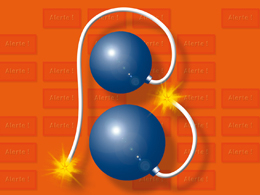
\includegraphics[width=3cm]{image/bonsai.jpg}
    \end{flushleft}
  \end{minipage}
  \begin{minipage}{0.4\textwidth}
    \begin{flushright} \large
      
\includegraphics[width=3cm]{image/lille1.png}
    \end{flushright}
  \end{minipage} 
  ~\\[3cm]

  \textsc{\LARGE PJI\\ Master 1 informatique}\\[1.5cm]

  \textsc{\Large Université Lille 1}\\[0.5cm]

  % Title
  \HRule \\[0.5 cm]
  { \huge \bfseries Prédiction de l'activité des peptides\\[0.8cm] \large \emph{CRISTAL - Equipe BONSAI} \\[0.4cm] }
  \HRule \\[1.5 cm]

  % Author and supervisor
  \begin{minipage}{0.4\textwidth}
    \begin{flushleft} \large
      \emph{Auteur:}\\
	Emilie \textsc{Allart}
    \end{flushleft}
  \end{minipage}
  \begin{minipage}{0.4\textwidth}
    \begin{flushright} \large
      \emph{Tuteurs:} \\
      Maude \textsc{Pupin} \\
      Laurent \textsc{Noé}
    \end{flushright}
  \end{minipage} 

  \\[3cm]
  {\large \emph{9 mars 2015} }
  \vfill
 \end{center}
\end{titlepage}

  \section*{Remerciements}
  
  ~~\\
  
  Je remercie Maude et Laurent pour m'avoir permis d'effectuer mon projet dans l'équipe Bonsai. 
  Merci de m'avoir suivie tout au long du développement de celui-ci, et de me laisser aller jusqu'au bout de mon projet en me donnant un stage.
  
  \phantomsection

  \addcontentsline{toc}{section}{Remerciements}
  \newpage
  
  \newpage
  \tableofcontents 
  \newpage

  \section*{Introduction}

      \paragraph
      \\
      ~~\\Au cours de la première année de master informatique, nous avons la possibilité de choisir dans le cadre du module PJI un projet à effectuer dans un laboratoire de recherche.
      J'ai donc effectué le mien au sein de l'équipe Bonsai, une équipe orientée bioinformatique faisant partie de CRISTAL. 
      
      ~~\\ Bonsai est un groupe de recherche en bioinformatique affilié avec INRIA Lille - Nord Europe et le Centre de Recherche en Informatique, Signal et Automate de Lille (CRIStAL, Université Lille 1, CNRS).
      Leur objectif principal est de définir des modèles et des algorithmes efficaces pour l'analyse de séquence à grande échelle dans le dommaine de la biologie moléculaire. Cela comprend par exemple la génomique comparative et la métagénomique .
      
      Une branche en particulier est orientée vers les peptides non ribosomiques (ou NRPs) dirigée par Maude Pupin.  
     
      C'est pourquoi, encadrée par Maude Pupin et Laurent Noé, j'ai travaillé sur le thème de : \textit{Rechercher les meilleurs critères pour la prediction de l'activité d'un peptide}.
      Ceci rejoint une étude menée auparavant par l'équipe, intitulée \textit{A new fingerprint to predict nonribosomal peptides acitvity}, qui étudie la décomposition d'un NRP en monomères (sous-ensemble) pour prédire son activité.
     
      Nous allons donc étudier les peptides de la base Norine et essayer de trouver de nouveaux critères pour améliorer la prédiction de l'activité d'un peptide. De plus, une automatisation du programme permettra aux personnes le souhaitant d'utiliser leur base d'apprentissage.
      ~~\\Le but est de pouvoir par la suite prédire l'activité d'un peptide inconnu, avec pour information sa composition en monomères et sa structure. Et d'améliorer potentiellement les résulats par rapport à la précédente recherche.
     
     
      ~~\\Dans ce rapport, nous allons expliquer ce qu'est un NRP et présenter Norine, puis annoncer le plan du projet. Dans une deuxième partie, nous détaillerons étape par étape le travail effectué. Enfin nous présenterons les résultats obtenus en réalisant une comparaison avec l'étude précédente, et les réponses que l'on peut en tirer.
     
      \addcontentsline{toc}{section}{Introduction}
      \newpage


  \chapter{Contexte}

    
    \section{NRP}
    

     
      \begin{minipage}[c]{\textwidth}
	\centering
	  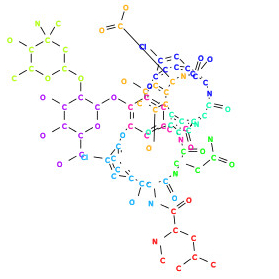
\includegraphics[width=5cm]{image/v.jpeg}
	  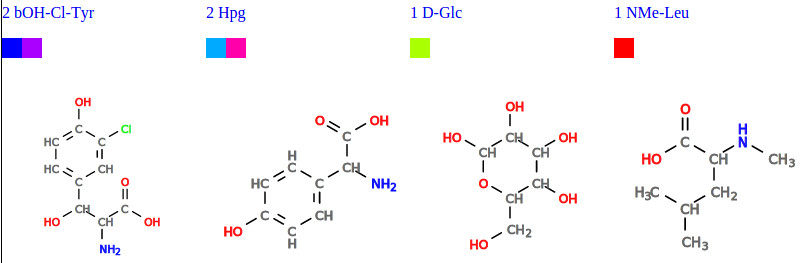
\includegraphics[width=10cm]{image/mono1.jpeg}
	  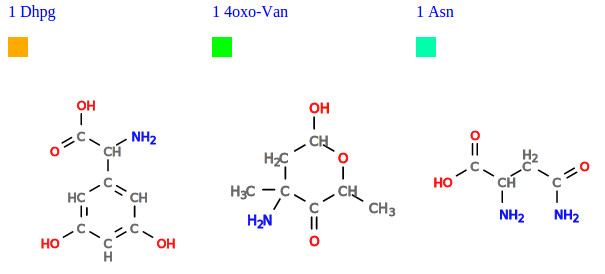
\includegraphics[width=10cm]{image/mono2.jpeg}
	  \captionof{figure}{Décomposition de la vancomycin en monomères}
	  \label{image1}
	\end{minipage}
	
	
    
 	~\\ 
	Les bactéries et les champignons comportent des peptides synthétisés par une voie indépendante du ribosome. 
	Ils ne suivent pas la voie classique allant de la transcription de l'ADN, à la traduction de l'ARN en peptide sur le ribosome.
	Ils utilisent une voie alternative utilisant des NRPSs (ou non-ribosomal peptide synthetase) qui sont des complexes multi-enzimatiques organisés en module.
	Les NRPs sont des composés chimiques synthétisés par de grandes enzymes qui regroupent des acides aminés mais aussi leur(s) dérivés ainsi que d'autres composés (des lipides ou des glucides par exemple). Ces composés sont associés par des liaisons peptidiques et non peptidiques. 
	
	\\Les NRPs servent déjà à fournir des médicaments mais leur capacité à fournir de nouveaux médicaments et produits pharmacologiques n'est pas encore assez exploitée. Il faut donc continuer à en découvrir de nouveaux et en apprendre d'avantage sur leurs activités.

      \subsection{Monomère}
	
	~~\\Pour mieux comprendre les NRPs, une décomposition en monomères a été mise en place. (cf figure 1.1) 
	Comme dit auparavant, un NRP est un assemblage d'acides aminés mais aussi de lipides et glucides, que nous  appelons monomères (les unités de base) . 
	Un NRP a la spécificité d'être de petite taille (2 à 50 monomères) et d'être fort diversifié car il existe plus de 500 monomères comptant les 21 acides aminés et tous leur(s) dérivés.
	Ainsi, on peut décrire un NRP par l'ensemble des monomères qui le composent et en tirer des informations. 
	
	\\Voici la décomposition monomérique de la vancomycin : Asn,bOH-Cl-Tyr,NMe-Leu,Hpg,D-Glc,Van,bOH-Cl-Tyr,Dhpg,Hpg
	
      \subsection{Structure}
	

	\begin{figure}[h]
	    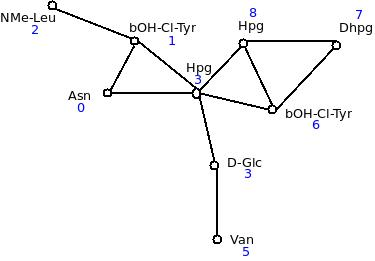
\includegraphics[scale = 0.5]{image/vanco_mono.jpeg}
	    \caption{Représentation graphique de la vancomycin }
	\end{figure}
	
	\begin{flushleft}
	  \begin{tabular}{|c|c|c|c|c|c|c|c|c|}\hline
	    \color{blue}0 & \color{blue}1 & \color{blue}2 & \color{blue}3 & \color{blue}4 & \color{blue}5 & \color{blue}6 & \color{blue}7 & \color{blue}8 \\\hline
	    Asn & bOH-Cl-Tyr & NMe-Leu & Hpg & D-Glc & Van & bOH-Cl-Tyr & Dhpg & Hpg \\\hline
	    @1,3 & @0,2,3 & @1 & @1,0,4,6,8 & @3,5 & @4 & @3,7,8 & @6,8 & @3,7,6 \\\hline
	  \end{tabular}
	  \captionof{table}{Représentation des liens entre les monomères composant la vancomycin}
	  \label{table0}
	 \end{flushleft}
	

	~~\\Il est plus aisé de représenter un NRP sous la forme d'un graphe avec pour noeuds les monomères qui le constituent, et pour liens les liaisons qui les relient.
	Le NRP ne contient pas seulement des liaisons peptidiques, mais également des liaisons non-peptidiques. Cela engendre donc l'apparition possible de structures cycliques (partielles ou non) et de ramifications sur la structure primaire de la molécule. 
	
	Grâce à la structure du NRP (graphe), on peut décrire les liens entre les monomères et analyser l'effet qu'ils ont sur l'activité du peptide.
	C'est pourquoi, dans le projet, l'arité de chaque monomère, c'est-à-dire le nombre de liaisons que possède un monomère, est étudié.
	
	On peut décrire cette structure par une description linéaire qui liste les monomères dans un ordre, permettant d'identifier un monomère par sa position, et à la suite, à l'aide de symboles '@', se trouve les liens qui existent entre eux
	
	\\Voici la description linéaire de la vancomycin : Asn,bOH-Cl-Tyr,NMe-Leu,Hpg,D-Glc,Van,bOH-Cl-Tyr,Dhpg,Hpg @1,3 @0,2,3 @1 @1,0,4,6,8 @3,5 @4 @3,7,8 @6,8 @3,7,6 
	
	\subsection{Activité}
	
	En effet, les NRPs sont une mine d'or pour les biologistes, ils ont un large domaine d'activité au niveau biologique et pharmacologique. 
	Ils peuvent, par exemple, avoir comme activité:
	\begin{itemize}
	 \item antibiotique : lutte contre les bactéries \textit{ex : ACV (précurseur de la penicilline)}  
	 \item anticancéreux : lutte contre le cancer \textit{ex : actinomycin D}
	 \item toxine :  tue les cellules \textit{ex :callipeltin D}
	 \item sidérophore : agit comme un aimant avec les molécules de fer \textit{ex : amphibactin I}
	 \item inhibiteur de la protéase : lutte contre les virus \textit{ex : cyanostatin B}
	\end{itemize}
	Un NRP peut posséder plusieurs activités à la fois, mais nous ne considerons, dans ce travail, que ceux qui ne possèdent qu'une seule activité.
       
      \subsection{Clusters}
	
	~\\
	Bien souvent les monomères partagent des propriétés physico-chimiques, soit parce qu'ils ont une structure similaire, soit parce qu'ils dérivent tous d'un même composant auquel s'est ajouté un groupement ( groupement acetyl, methyl, etc...), ou qui a changé de conformité. Cela nous permet de les ranger dans des clusters (ou des familles).
	
	Ainsi, nous examinons ces clusters et regardons s'ils peuvent nous aider à améliorer la prediction de l'activité d'un peptide.
	
	Voici une sous-partie des clusters que nous avons utilisée :
	
	\begin{description}
	 \item[Chromophores non siderophore] \hfill \\ChrD;ChrA;ChrAct
	 \item[Siderophores] \hfill \\ChrI;ChrP;OH-Asp;D-OH-Asp;OH-His;Ac-OH-Orn;D-Fo-OH-Orn;D-OH-Orn;D-Ac-OH-Orn;D-OH-cOrn;OH-Orn;NAc-Fo-OH-Orn;Fo-OH-Orn;OH-cOrn
	 \item[Peptaibols (antibiotiques)]\hfill \\ NAc-Dpr;Ac-Ser;Ac-Ival;Ac-Val;Ac-Trp;Ac-Phe;Ac-Aib;NAc-Leu;Ivalol;Leuol;Valol;Ileol;Pheol;Trpol;Serol;OAc-Leuol;Aib;Ival;4OH-Pro;Et-Nva
	 \item[Hpg et derives (antibiotiques)] \hfill \\Hpg;D-OH-dHpg;Cl2-Hpg;NMe-Hpg;Cl-Hpg;OH-dHpg;D-Hpg
	 \item[Sucres (antibiotiques)] \hfill \\2OMe-Rha;Ara;Aco;D-Gal;D-Ara;Ere;Glc;Oli;D-Glc;bD-Gal;U4oxo-Van;Rha;D-Man;4oxo-Van;Act;Lyx;Ria;Van
	\end{description}

	
	  
      \section{Norine}
	 ~\\
	 \begin{minipage}[c]{\textwidth}
	    \centering
	     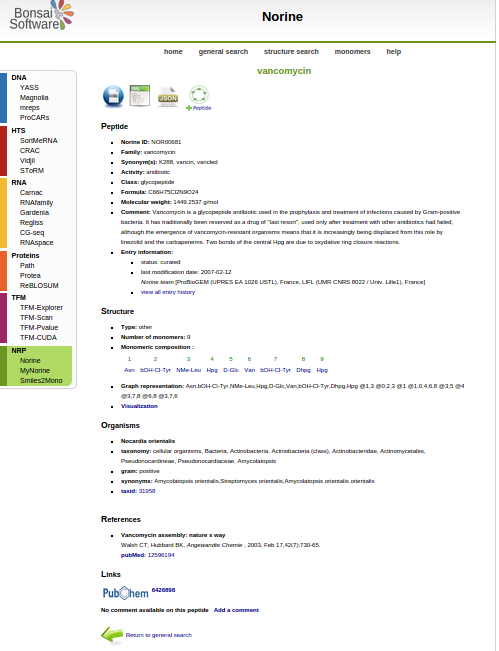
\includegraphics[scale =0.7]{image/Norine.png}
	      \caption{Capture de la description d'un peptide sur Norine}
	 \end{minipage}
	 
	  \paragraph{}

	  \\Norine (NOnRibosomal peptides with INE) est une plateforme contenant la première base de données entièrement dédiée aux peptides non ribosomiques, elle répertorie 1174 NRPs et pas moins de 528 monomères. Elle fournit aussi les outils permettant le traitement de ces NRPs. 
	  Le site est organisé en plusieurs parties, une partie 'peptide' présente pour un peptide donné son nom, ses synonymes, les activités biologiques, sa formule moléculaire, sa formule monomérique , etc...; une autre partie 'structure' où l'on retrouve les peptides classés par type (cyclique, linéaire, double cyclique, ...), qui donne la structure monomérique des peptides.
	  On peut également trouver la description des monomères. 
	  Voici ci-dessus le résultat rendu pour une recherche sur la vancomycin.
	
	
	
      \section{Problématique}
	
	\paragraph{}
	  Les NRPSs , bien que fort intéressants, sont difficile à produire et à analyser. On ne peut donc pas utiliser les méthodes habituelles d'analyse de forme 3D ou de leur reaction physico-chimique.
	  C'est pourquoi le but de l'étude précédente est de donner des modèles de prediction informatique permettant de prédire l'activité d'un peptide.
	  Ces modèles se basaient uniquement sur l'empreinte monomérique du peptide, c'est-à-dire un comptage de chaque monomère pour voir lesquels sont présents et en déterminer d'après l'apprentissage quel 'schéma' ils suivent.

	  Pour notre part , nous ajouterons d'autres critères, à savoir l'occurence des clusters de monomères et le comptage des liens.
	  Puis, par le biais de méthodes d'apprentissage et de validation croisée, nous chercherons à voir lequel ou lesquels de ces critères prédisent au mieux l'activité du peptide concerné.
	  
	  Dans l'idéal, nous aurons de meilleurs modèles pour prédire l'activité d'un peptide. Nous comparerons les différents résulats entre eux et avec ceux de la précédente étude, pour trouver les meilleurs critères.
	
	
      \section{Plan}
	
	
	  \begin{figure}[hl]
	    \leftskip -2cm
	    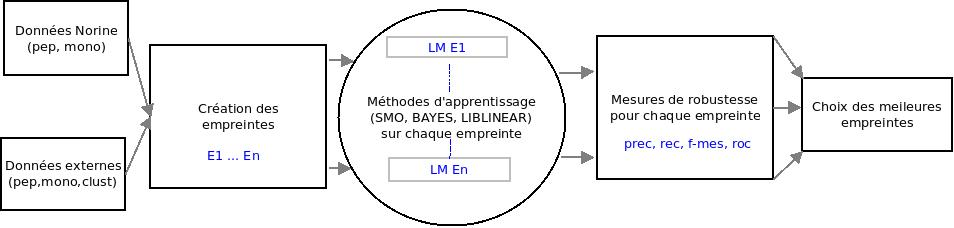
\includegraphics[scale = 0.5]{image/Plan.jpeg}
	    \caption{Schéma des étapes à suivre}
	  \end{figure}
	
	  \\ Ce schéma énonce le principe du projet, tout d'abord nous prélevons les données de Norine ou nous joignons des fichiers de données, puis nous créons nos empreintes.  
	  Ces empreintes sont ensuite analysées par des méthodes d'apprentissage, nous donnant ainsi de métriques de qualité que nous comparons pour voir quelles empreintes apportent de bonnes connaissances.
	  
   
  \chapter{Mise en oeuvre}

  
    \section{Récupération depuis Norine}
    
	\begin{figure}[!h]
	    \begin{center}
	      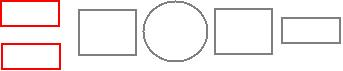
\includegraphics[width=5cm]{image/step1.jpeg} \\
	      \caption{Schéma de l'avancée}
	    \end{center}
	 \end{figure}
	   
	\\
	Norine met à diposition une passerelle REST, nous permettant de récupérer plus facilement les données.
	De cette façon, par l'intermédiaire de fichier JSON, nous avons récupéré les informations sur chaque peptide nous intéressant, ainsi que la liste de tous les monomères de la base.
	
	    
	~\\ Sur chaque peptide, si toutes les données sont fournies, nous conservons son identifiant (représenté parles lettres NOR suivies de 5 chiffres), sa composition monomérique, son activité et sa structure linéaire. 
	    
	Pour rester cohérent avec l'étude précédente, nous avons enlevé une activité redondante nommée 'surfactant' et nous ne conservons que les peptides ayant une seule activité.
	Nous avons également créé un filtre qui ne garde que les peptides dont l'activité est assez représentative, le nombre de peptides possédant chacune de ces activités doit dépasser un certain seuil que nous fixons préalablement. Pour notre étude, nous avons fixé ce seuil à 20 peptides.
      
	Une fois les données récupérées, nous les traitons selon les critères que nous souhaitons tester.   
   
    \section{Création des empreintes}
	
	\begin{figure}[!h]
	    \begin{center}
	      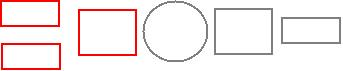
\includegraphics[width=5cm]{image/step2.jpeg} \\
	      \caption{Schéma de l'avancée}
	    \end{center}
	 \end{figure}
	 
	Une fois les données récupérées de Norine et filtrées, nous réalisons les empreintes.
	
	\paragraph{Empreinte en monomère}
	    ~\\
	    Au préalable nous avons prélevé l'ensemble des monomères de Norine. Mais il est possible pour une personne souhaitant utiliser ses données de donner au programme un fichier contenant les monomères qu'il a répertoriés.
	    
	    A chaque peptide, nous comptons le nombre d'occurences de chaque monomère dans sa composition et en faisons ainsi une empreinte.
	    
	   \begin{figure}[h]
	    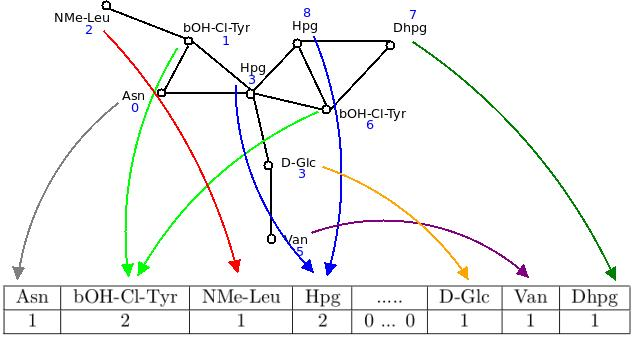
\includegraphics[scale = 0.5]{image/vanco_monoB.jpeg}
	    \caption{Schéma montrant la création des empreintes en monomères}
	    \end{figure}
	
	    
	\paragraph{Empreinte en cluster}
	~\\
	  De même que pour les monomères, nous devons au préalable charger un fichier répertoriant les clusters de monomères avec leur nom et les monomères qui les composent.
	  
	  C'est le même principe qu'auparavant, nous faisons l'empreinte mais cette fois nous notons le nombre d'occurences d'un cluster en comptant combien de fois les éléments de celui-ci apparaissent dans ce peptide.
	 
	  
	\paragraph{Empreinte en lien}
	    ~\\
	    Comme dit précédemment, les NRPs sont représentés par des graphes de monomères. On peut donc intégrer la notion d'arité, qui représente le nombre de lien que possède un sommet, donc pour notre problème, cela représente le nombre de monomères auquel est lié un monomère. 
	    Pour chaque arité, allant de 1 à 5, nous comptons le nombre de sommets ayant cette arité, et l'ajoutons à notre empreinte.

	\paragraph{}
	  ~\\
	  Selon les critères que nous voulons tester, nous ajoutons à la liste pour chaque peptide leur(s) empreinte(s).
	  Nous pouvons ainsi tester les critères, chacun pris séparément ou combinés : par exemple les liens et les monomères ensemble ou alors les clusters seuls.
	  
     \section{Lancement des méthodes d'apprentissage}
     
	  \begin{figure}[!h]
	    \begin{center}
	      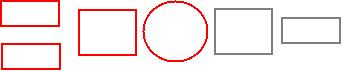
\includegraphics[width=5cm]{image/step3.jpeg} \\
	      \caption{Schéma de l'avancée}
	    \end{center}
	 \end{figure}
	  
	  ~\\
	  Pour traiter les données, nous utilisons 3 méthodes d'apprentissage : le NaïveBayes, le SMO et le LibLinear. 
	  
	  Pour cela, nous avons utilisé des librairies python et une extension pour LibLinear qui n'est pas implémentée de base.
	  
	  ~\\Le Naïve Bayes repose sur le théorème de Bayes, il possède une phase d'entrainement et une phase de test.
	  Puis, on fait de l'apprentissage probabiliste sur l'ensemble des peptides, ainsi lorsque l'on teste à quelle activité appartient un nouveau peptide, on conserve la classe qui a la plus grande probabilité.  
	    
	  Le SMO est une méthode d'apprentissage supervisé qui construit, au fur et à mesure de la lecture des données, une fonction objective via une descente de gradient.   
	  LibLinear reste dans la même idée.
	      
	  \paragraph{Validation croisée}
	    
	  Nous divisons les peptides en 10 groupes, nous faisons un apprentissage des empreintes sur 9 groupes et testons sur le dernier groupe si l'activité que l'on trouve correspond bien. Nous faisons cela pour chacun des groupes et obtenons ainsi des mesures de qualités.
	    
     \section{Mesures de robustesse}
     
	  \begin{figure}[!h]
	    \begin{center}
	      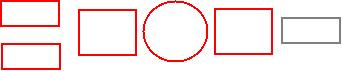
\includegraphics[width=5cm]{image/step4.jpeg} \\
	      \caption{Schéma de l'avancée}
	    \end{center}
	 \end{figure}
	  
	  ~\\
	  Nous obtenons ainsi un ensemble de mesures de robustesse qu'il faut comparer pour voir quel critère ou quelel combinaison de critères est le/la plus efficace pour obtenir des informations sur un peptide.
	  Pour notre étude, nous utilisons la précision, la sensibilité, l'acc, la F-measure et le ROC.
	  
	  \begin{figure}[!h]
	    \begin{center}
	      \leftskip -4cm
	      \includegraphics[width=20cm]{image/measure.jpeg} \\
	      \caption{Tableau résumant les différentes mesures}
	    \end{center}
	  \end{figure}
	  
	     \paragraph{Precision}\\
	      
	     ~\\ 
	     Aussi appelée PPV (Positive Predictive Value), la précision se calcule en divisant le nombre d'éléments bien rangés dans une classe par le nombre d'éléments rangés dans cette classe.
	     Dans notre cas, elle se calcule en divisant le nombre de peptides bien classés pour une activité par le nombre de peptides classés pour cette activité.
	     Elle est la probabilité que les données soient bien triées, une mesure de la qualité de la classification. 
	     Donc un taux élevé est attendu dans la recherche.
	     \[ 
	      précision = \frac{ TP }{ TP + FP }
	     \]

	     
	     \paragraph{Sensibilité}
	     
	     ~\\
	     La sensibilité, que l'on appelle aussi recall ou TPR(True Positive Rate) se calcule en divisant le nombre d'éléments bien classés par le test pour une classe donnée sur le nombre de données qui devraient être dans cette classe. 
	     Cela représente le nombre de peptides bien annotés pour une activité par rapport au nombre de peptides possédant cette activité.
	     Elle prend une valeur entre 0 et 1, plus elle tend vers 1 plus la classification est bonne.
	     \[
	      sensibilite = \frac{ TP }{ TP + FN }
	     \]

	     \paragraph{F-measure}\\
	     
	     ~\\La F-measure allie la précision et la sensibilité, ainsi si elle approche 1 c'est un bon résulat.
	     \[
	      f-measure = \frac{ 2 \times precision \times sensibilite }{ precision + sensibilite }
	     \]
	     \paragraph{AUC ou ROC}\\
		
	     ~\\La courbe ROC est la courbe représentant le TPR (True Positif Rate) en fonction du FPR (False Positif Rate), elle permet de visualiser les données bien classées par rapport aux données mal classées.
	     L'AUC, signifiant Area Under Curve, est égal à la probabilité qu'une donnée choisie au hasard ait plus de chance d'être classée positive que négative.
	     
	     \paragraph{ACC}
	     
	     ~\\Abbréviation pour Accuracy, elle permet de connaitre le ratio de données bien classées sur l'ensemble des données.
	     C'est le nombre de peptides bien classés sur le nombre total des peptides.
	     \[
	      ACC = \frac{ TP + TN }{ P + N }
	     \]
	     
	     
   \chapter{Résultats}
      
      \begin{figure}[!h]
	    \begin{center}
	      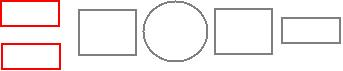
\includegraphics[width=5cm]{image/step1.jpeg} \\
	      \caption{Schéma de l'avancée}
	    \end{center}
	 \end{figure}
      
       \section{Comparaison avec les résultats précédents}
      
	  \paragraph{} 
	   \begin{flushleft}
	    \leftskip -3cm
	    \begin{tabular}{|c||c|c|c|c||c|c|c|c||c|c|c|c|}\hline
	      {Activite} & \multicolumn{4}{c||}{Naive Bayes} & \multicolumn{4}{c||}{LibLinear} & \multicolumn{4}{c|}{SMO} \\\cline{2-13}
	       & Prec & Rec & F & AUC & Prec & Rec & F & AUC & Prec & Rec & F & AUC \\\hline
	      Antibiotique & 0,971 & 0,737 & 0,838 & 0,961 & 0,950 & 0,962 & 0,956 & 0,953 & 0,947 & 0,953 & 0,950 & 0,942 \\\hline
	      Toxine & 0,656 & 0,898 & 0,758 & 0,946 & 0,899 & 0,904 & 0,902 & 0,934 & 0,889 & 0,917 & 0,902 & 0,937  \\\hline
	      Siderophore & 0,890 & 0,988 & 0,936 & 0,998 & 0,988 & 0,963 & 0,975 & 0,981 & 1 & 0,951 & 0,975 & 0,994  \\\hline
	      Anticancereux & 0,471 & 0,640 & 0,542 & 0,935 & 0,696 & 0,640 & 0,667 & 0,814 & 0,696 & 0,640 & 0,667 & 0,868 \\\hline
	      Inhibiteur protease & 0,870 & 0,909 & 0,889 & 0,996 & 0,952 & 0,909 & 0,930 & 0,954 & 0,952 & 0,909 & 0,930 & 0,975 \\\hline
	      Accuracy & \multicolumn{4}{l||}{81,49} & \multicolumn{4}{l||}{93,22} & \multicolumn{4}{l|}{92,89} \\\hline
	    \end{tabular}
	     \captionof{table}{Mesures de robustesse de l'apprentissage de l'étude précédente}
	     \label{tableau 1}
	  \end{flushleft}
	  
	  
	   \begin{flushleft}
	    \leftskip -3cm
	    \begin{tabular}{|c||c|c|c|c||c|c|c|c||c|c|c|c|}\hline
	      {Activite} & \multicolumn{4}{c||}{Naive Bayes} & \multicolumn{4}{c||}{LibLinear} & \multicolumn{4}{c|}{SMO} \\\cline{2-13}
	       & Prec & Rec & F & AUC & Prec & Rec & F & AUC & Prec & Rec & F & AUC \\\hline
	      Antibiotique & 0,967 & 0,794 & 0,872 & 0,956 & . & . & . & . & 0,947 & 0,960 & 0,954 & 0,941 \\\hline
	      Toxine & 0,742 & 0,803 & 0,771 & 0,958 & . & . & . & . & 0,834 & 0,925 & 0,877 & 0,955  \\\hline
	      Siderophore & 0,719 & 0,967 & 0,825 & 0,995 & . & . & . & . & 0,967 & 0,967 & 0,967 & 0,990  \\\hline
	      Anticancereux & 0,311 & 0,576 & 0,404 & 0,898 & . & . & . & . & 0,765 & 0,394 & 0,520 & 0,764 \\\hline
	      Inhibiteur protease & 0,660 & 0,921 & 0,769 & 0,989 & . & . & . & . & 0,903 & 0,737 & 0,812 & 0,960 \\\hline
	      Accuracy & \multicolumn{4}{l||}{81,24} & \multicolumn{4}{l||}{.} & \multicolumn{4}{l|}{92,02} \\\hline
	    \end{tabular}
	     \captionof{table}{Mesures de robustesse de l'apprentissage sur l'empreinte monomérique}
	     \label{table 2}
	  \end{flushleft}
	  
	 \\
	 En partant des mêmes données que l'étude précédente, c'est-à-dire une seule activité en omettant les surfactants et avec un seuil d'activité à 20, nous pouvons voir que les résultats obtenus sur les empreintes monomériques sont similaires.
	 Nous sommes donc partis pour notre étude sur les mêmes bases que la précédente.
	 
	 
      \section{Résultats obtenus}
	 
	  Voici un résumé des meilleurs résultats obtenus lors de la recherche, les empreintes de clusters et des liens seuls n'étant pas représentatifs, ils ne sont pas présentés dans le document.
	  Ayant rencontré des problèmes dans le lancement de LibLinear sur les données, les résultats ne sont pas présentés non plus.
	
	  \begin{flushleft}
	    \leftskip -3cm
	    \begin{tabular}{|c||c|c|c|c||c|c|c|c||c|c|c|c|}\hline
	      {Activite} & \multicolumn{4}{c||}{Naive Bayes} & \multicolumn{4}{c||}{LibLinear} & \multicolumn{4}{c|}{SMO} \\\cline{2-13}
	      & Prec & Rec & F & AUC & Prec & Rec & F & AUC & Prec & Rec & F & AUC \\\hline
	      Antibiotique & 0,970 & 0,794 & 0,873 & 0,959 & . & . & . & . & 0,953 & 0,965 & 0,959 & 0,949 \\\hline
	      Toxine & 0,748 & 0,810 & 0,778 & 0,962 & . & . & . & . & 0,860 & 0,918 & 0,888 & 0,954 \\\hline
	      Siderophore & 0,759 & 0,978 & 0,854 & 0,997 & . & . & . & . & 1,000 & 0,967 & 0,983 & 0,994  \\\hline
	      Anticancereux & 0,373 & 0,576 & 0,452 & 0,912 & . & . & . & . & 0,739 & 0,515 & 0,607 & 0,836  \\\hline
	      Inhibiteur protease & 0,507 & 0,921 & 0,654 & 0,994 & . & . & . & . & 0,914 & 0,842 & 0,877 & 0,979 \\\hline
	      Accuracy & \multicolumn{4}{l||}{81,50} & \multicolumn{4}{l||}{.} & \multicolumn{4}{l|}{93,16} \\\hline
	    \end{tabular}
	     \captionof{table}{Mesures de robustesse de l'apprentissage sur l'empreinte de monomères-liens}
	     \label{table 3}
	  \end{flushleft}
	  
	  \\ Si nous comparons les résultats de l'empreinte monomères-liens aux résultats précédents, le SMO nous montre des résultats plus élevés. 
	  D'après cela, l'association monomères-liens nous apporterait plus d'information pour la détermination de l'activité d'un peptide.

	   \begin{flushleft}
	    \leftskip -3cm
	    \begin{tabular}{|c||c|c|c|c||c|c|c|c||c|c|c|c|}\hline
	      {Activite} & \multicolumn{4}{c||}{Naive Bayes} & \multicolumn{4}{c||}{LibLinear} & \multicolumn{4}{c|}{SMO} \\\cline{2-13}
	      & Prec & Rec & F & AUC & Prec & Rec & F & AUC & Prec & Rec & F & AUC \\\hline
	      Antibiotique & 0,976 & 0,759 & 0,854 & 0,957 & . & . & . & . & 0,953 & 0,965 & 0,959 & 0,947 \\\hline
	      Toxine & 0,677  & 0,857 & 0,757 & 0,957 & . & . & . & . & 0,834 & 0,925 & 0,877 & 0,949  \\\hline
	      Siderophore & 0,798 & 0,967 & 0,874 & 0,995 & . & . & . & . & 0,989 & 0,967 & 0,978 & 0,979  \\\hline
	      Anticancereux & 0,313 & 0,606 & 0,412 & 0,896 & . & . & . & . & 0,750 & 0,455 & 0,566 & 0,773 \\\hline
	      Inhibiteur protease & 0,625 & 0,921 & 0,745 & 0,988 & . & . & . & . & 0,903 & 0,737 & 0,812 & 0,964 \\\hline
	      Accuracy & \multicolumn{4}{l||}{80,23} & \multicolumn{4}{l||}{.} & \multicolumn{4}{l|}{92,52} \\\hline
	    \end{tabular}
	     \captionof{table}{Mesures de robustesse de l'apprentissage sur l'empreinte de monomères-clusters}
	     \label{table 4}
	  \end{flushleft}
	  	
	  \\ En ce qui concerne l'empreinte monomères-clusters, l'information est intéressante pour les deux premières classes qui sont les plus représentatives des données, mais nous apporte moins d'information par rapport aux précédents résultats sur les autres activités.
	  Donc l'association monomères-clusters n'est pas vraiment intéressante pour la prédiction.
	  	  
	  \begin{flushleft}
	    \leftskip -3cm
	    \begin{tabular}{|c||c|c|c|c||c|c|c|c||c|c|c|c|}\hline
	      {Activite} & \multicolumn{4}{c||}{Naive Bayes} & \multicolumn{4}{c||}{LibLinear} & \multicolumn{4}{c|}{SMO} \\\cline{2-13}
	      & Prec & Rec & F & AUC & Prec & Rec & F & AUC & Prec & Rec & F & AUC \\\hline
	      Antibiotique & 0,966 & 0,649 & 0,776 & 0,858  & . & . & . & . & 0,687 & 0,996 & 0,813 & 0,644 \\\hline
	      Toxine & 0,417 & 0,769 & 0,541 & 0,831 & . & . & . & . & 0,400 & 0,014 & 0,026 & 0,584  \\\hline
	      Siderophore & 0,889 & 0,978 & 0,931 & 0,998 & . & . & . & . & 1,000 & 0,967 &  0,983 & 0,996  \\\hline
	      Anticancereux & 0,000 & 0,000 & 0,000 & 0,824 & . & . & . & . & 0,000 & 0,000 & 0,000 & 0,784 \\\hline
	      Inhibiteur protease & 0,402  & 0,974 & 0,569 & 0,972 & . & . & . & . & 0,000 & 0,000 & 0,000 & 0,743\\\hline
	      Accuracy & \multicolumn{4}{l||}{69,71} & \multicolumn{4}{l||}{.} & \multicolumn{4}{l|}{71,99} \\\hline
	    \end{tabular}
	     \captionof{table}{Mesures de robustesse de l'apprentissage sur l'empreinte de clusters-liens}
	     \label{table 5}
	  \end{flushleft}
	   
	   \\ Il en va de même pour l'empreinte clusters-liens, on peut voir que l'apport d'information est plus faible par rapport aux précédentes empreintes, elle n'est donc pas à retenir. 
	  
	   \begin{flushleft}
	    \leftskip -3cm
	    \begin{tabular}{|c||c|c|c|c||c|c|c|c||c|c|c|c|}\hline
	      {Activite} & \multicolumn{4}{c||}{Naive Bayes} & \multicolumn{4}{c||}{LibLinear} & \multicolumn{4}{c|}{SMO} \\\cline{2-13}
	      & Prec & Rec & F & AUC & Prec & Rec & F & AUC & Prec & Rec & F & AUC \\\hline
	      Antibiotique &  0,973 & 0,757 & 0,851 & 0,960 & . & . & . & . & 0,957 & 0,965 & 0,961 & 0,952 \\\hline
	      Toxine & 0,723 & 0,816 & 0,767 & 0,962 & . & . & . & . & 0,854 & 0,918 & 0,885 & 0,956  \\\hline
	      Siderophore & 0,784 & 0,967 & 0,866 & 0,997 & . & . & . & . & 1,000 & 0,967 & 0,983 & 0,996  \\\hline
	      Anticancereux & 0,308 & 0,606 & 0,408 & 0,911 & . & . & . & . & 0,708 & 0,515 & 0,596 & 0,828 \\\hline
	      Inhibiteur protease & 0,479 & 0,921 & 0,631 & 0,992 & . & . & . & . & 0,914  & 0,842 & 0,877 & 0,977 \\\hline
	      Accuracy & \multicolumn{4}{l||}{79,34} & \multicolumn{4}{l||}{.} & \multicolumn{4}{l|}{93.16} \\\hline
	    \end{tabular}
	     \captionof{table}{Mesures de robustesse de l'apprentissage sur l'empreinte de monomères-clusters-liens}
	     \label{table 6}
	  \end{flushleft}
	  
	  \\ Pour finir, l'empreinte comprenant l'ensemble des données apporte très peu d'information supplémentaire, cela doit être dû au peu d'information qu'apporte l'empreinte en cluster.

	  
	  
	  \\ Par conséquent, l'étude a montré que l'empreinte monomères-liens pourrait être un bon critère pour la prédiction de l'activité d'un peptide.
	     Pour s'en assurer, il faudra par la suite obtenir les résultats de la méthode LibLinear.
	     
      
     
  \section*{Conclusion}
     
    \phantomsection
    \addcontentsline{toc}{section}{Conclusion}
    \newpage

    Pour rappel, notre problématique était de chercher de meilleurs critères pour déterminer l'activité d'un peptide. 
    A savoir que le programme est conçu pour que toute personne le souhaitant puisse faire l'apprentissage sur ses propres données.

   
    En comparant, les résulats de l'étude effectuée sur les NRPs de Norine quelques années auparavant et les résultats que nous avons obtenus en combinant différentes connaissances sur ces NRPs, nous avons trouvé des combinaisons de critères nous permettant d'apprendre avec plus de certitudes l'activité d'un NRP. 
    Pour connaitre l'activité d'un NRP avec d'avantage de précision, il faut combiner l'empreinte en monomères et l'empreinte en liens.
    
    Pour pouvoir achever ce projet, il faudra obtenir les résultats de LibLinear, ceci sera fait lors de mon stage d'été avec, en parallèle, l'insertion de ce programme à Norine.
    
    
    \newpage

   
    \section*{Références}
     \end{itemize}

      \paragraph{}
      \begin{description}
       \item [Mesures de robustesse de Wikipédia :]
	\url{https://en.wikipedia.org/wiki/Receiver_operating_characteristic}
	
	\item [Norine :] 
	  \url{http://bioinfo.lifl.fr/norine/}
	
	\item [Maude Pupin :]
	  \url {http://www.lifl.fr/~pupin/research.html}
	 
	\item [NaiveBayes :]
	  \url {http://en.wikipedia.org/wiki/Naive_Bayes_classifier}\\
	  \url {https://weka.wikispaces.com/Programmatic+Use}
	
	\item [SMO :] 
	  \url{https://weka.wikispaces.com/Optimizing+parameters}
	
	\item [Liblinear :]
	  \utl {http://www.csie.ntu.edu.tw/~cjlin/liblinear/}
	  
	\end{description}
	\begin{thebibliography}{9}
      
	\bibitem{Art1}
	  S. Caboche, V. Leclère, M. Pupin, G. Kucherov, and P. Jacques
	  \emph{\LaTeX : Diversity of Monomers in Nonribosomal Peptides : towards the Prediction of Origin and Biological Activity}
	  Journal of Bacteriology,
	  2010
	 
	\bibitem{Art2}
	  A. Abdo, S. Caboche, V. Leclère, P. Jacques, and M. Pupin
	  \emph{\LaTeX :A new fingerprint to predict nonribosomal peptides activity }
	  J COmput Aided Mol Des,
	  2012
	  
	 \bibitem{Art3}
	 S. Caboche, M. Pupin, V. Leclère, A. Fontaine, P. Jacques, and G. Kucherov
	 \emph{\LaTeX : NORINE : a database of nonribosomal peptides}
	 Nucleic Acids Resaerch,
	 2007
	 
	 \bibitem{Art4}
	 Yoann DUFRESN, Valerie LECLERE, Philippe JACQUES, Laurent NOE, Maude PUPIN
	 \emph{\LaTeX : Non Ribosomal Peptides : A monomeric puzzle}
	 Conférence JOBIM,
	 2013
     \end{thebibliography}
     
     
    \phantomsection
    \addcontentsline{toc}{section}{Annexe}
    \newpage

    

  \end{document}          
